% fig_67_phasor.tex
% TR-32: Phasor diagram showing 67N/67Q forward vs reverse discrimination
%
% For X/R=20 network (arg(Z0S) ≈ 87°):
%   I0_forward  angle ≈ -87°  (slightly off -90°, mostly negative imaginary)
%   V0_forward  angle ≈ 180°  (negative real, with tiny neg imaginary component)
%   I0_reverse  angle ≈ +93°  (reversed at CT)
%   V0_reverse  angle ≈ 180°  (same bus voltage)
%
%   -V0  angle ≈ 0°  (positive real, tiny positive imaginary)
%   Operating zone: angle between -V0 and I0 within ±90°
%   Forward: angle(-87° to 0°) = -87° → within ±90° → TRIP
%   Reverse: angle(93° to 0°)  = +93° → outside ±90° → BLOCK
%
% Two sub-figures: left = forward fault, right = reverse fault

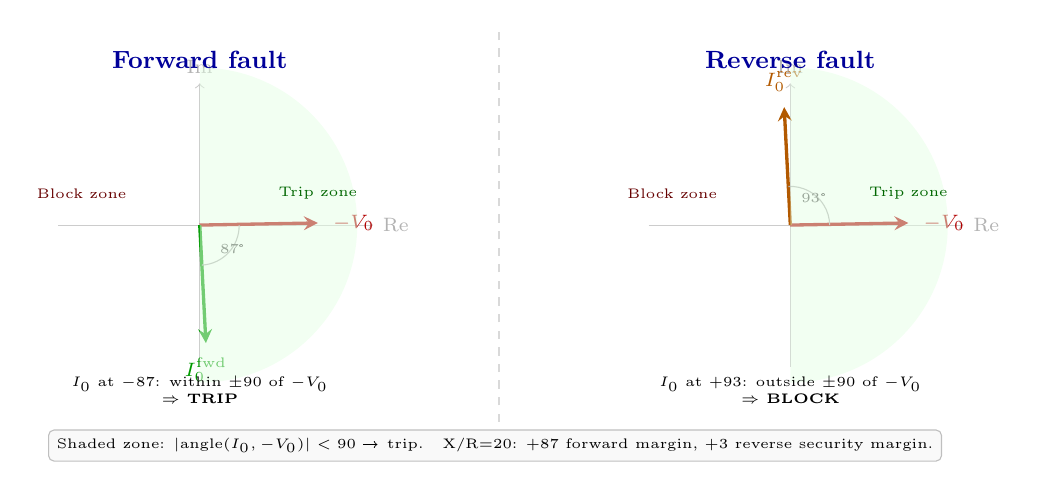
\begin{tikzpicture}[
  every node/.style = {font=\scriptsize},
  vec/.style        = {->, very thick, >=stealth},
  arc/.style        = {draw, thin, gray!60},
]

%% ── Shared scale: 1 unit = normalized phasor length ──────────────────────
\def\Rx{3.5}     % subplot separation
\def\Vs{1.5}     % vector scale

% ── LEFT SUBPLOT: FORWARD FAULT ─────────────────────────────────────────────
\def\ox{0}  \def\oy{0}

% Axes
\draw[gray!40, ->] (\ox-1.8, \oy) -- (\ox+2.2, \oy) node[right,gray!60]{Re};
\draw[gray!40, ->] (\ox, \oy-1.8) -- (\ox, \oy+1.8) node[above,gray!60]{Im};

% -V0 phasor: angle ≈ 0° (positive real, tiny +Im)
\draw[vec, red!70!black]
  (\ox,\oy) -- (\ox+\Vs*0.9998, \oy+\Vs*0.018);
\node[red!70!black, right=2pt] at (\ox+\Vs*0.9998, \oy+\Vs*0.018) {$-V_0$};

% I0 forward phasor: angle ≈ -87° (mostly -Im, tiny +Re)
\draw[vec, green!60!black]
  (\ox,\oy) -- (\ox+\Vs*0.052, \oy-\Vs*0.999);
\node[green!60!black, below=2pt] at (\ox+\Vs*0.052, \oy-\Vs*0.999) {$I_0^\mathrm{fwd}$};

% Arc showing angle between -V0 and I0: ≈ 87°
\draw[arc] (\ox+0.5,\oy) arc[start angle=1, end angle=-87, radius=0.5];
\node[gray!60!black, font=\tiny] at (\ox+0.42, \oy-0.30) {87°};

% Shading: operating zone (±90° of -V0)
\fill[green!10, opacity=0.5]
  (\ox,\oy) -- (\ox, \oy-2.0) arc[start angle=-90, end angle=90, radius=2.0] -- cycle;
\node[green!40!black, font=\tiny] at (\ox+1.5, \oy+0.4) {Trip zone};
\node[red!40!black, font=\tiny] at (\ox-1.5, \oy+0.4) {Block zone};

% Label
\node[font=\small, blue!60!black] at (\ox, \oy+2.1) {\textbf{Forward fault}};
\node[font=\tiny, align=center] at (\ox, \oy-2.1)
  {$I_0$ at $-87°$: within $\pm90°$ of $-V_0$\\$\Rightarrow$ \textbf{TRIP}};

% ── RIGHT SUBPLOT: REVERSE FAULT ────────────────────────────────────────────
\def\ox{7.5}

% Axes
\draw[gray!40, ->] (\ox-1.8, \oy) -- (\ox+2.2, \oy) node[right,gray!60]{Re};
\draw[gray!40, ->] (\ox, \oy-1.8) -- (\ox, \oy+1.8) node[above,gray!60]{Im};

% -V0 phasor: same as forward (bus voltage polarity unchanged)
\draw[vec, red!70!black]
  (\ox,\oy) -- (\ox+\Vs*0.9998, \oy+\Vs*0.018);
\node[red!70!black, right=2pt] at (\ox+\Vs*0.9998, \oy+\Vs*0.018) {$-V_0$};

% I0 reverse phasor: angle ≈ +93° (direction reversed at CT)
\draw[vec, orange!70!black]
  (\ox,\oy) -- (\ox-\Vs*0.052, \oy+\Vs*0.999);
\node[orange!70!black, above=2pt] at (\ox-\Vs*0.052, \oy+\Vs*0.999) {$I_0^\mathrm{rev}$};

% Arc: angle ≈ 93°
\draw[arc] (\ox+0.5,\oy) arc[start angle=1, end angle=93, radius=0.5];
\node[gray!60!black, font=\tiny] at (\ox+0.30, \oy+0.35) {93°};

% Shading: operating zone
\fill[green!10, opacity=0.5]
  (\ox,\oy) -- (\ox, \oy-2.0) arc[start angle=-90, end angle=90, radius=2.0] -- cycle;
\node[green!40!black, font=\tiny] at (\ox+1.5, \oy+0.4) {Trip zone};
\node[red!40!black, font=\tiny] at (\ox-1.5, \oy+0.4) {Block zone};

% Label
\node[font=\small, blue!60!black] at (\ox, \oy+2.1) {\textbf{Reverse fault}};
\node[font=\tiny, align=center] at (\ox, \oy-2.1)
  {$I_0$ at $+93°$: outside $\pm90°$ of $-V_0$\\$\Rightarrow$ \textbf{BLOCK}};

%% ── Divider ──────────────────────────────────────────────────────────────
\draw[gray!30, dashed] (3.8, -2.5) -- (3.8, 2.5);

%% ── Caption note ─────────────────────────────────────────────────────────
\node[draw=gray!50, fill=gray!5, rounded corners=2pt,
      font=\tiny, inner sep=3pt, align=center]
  at (3.75, -2.8)
  {Shaded zone: $|$angle$(I_0, -V_0)| < 90°$ → trip.\quad
   X/R=20: $+87°$ forward margin, $+3°$ reverse security margin.};

\end{tikzpicture}
